% Created 2017-06-07 Wed 09:43
% Intended LaTeX compiler: pdflatex
\documentclass[11pt]{article}
\usepackage[utf8]{inputenc}
\usepackage[T1]{fontenc}
\usepackage{graphicx}
\usepackage{grffile}
\usepackage{longtable}
\usepackage{wrapfig}
\usepackage{rotating}
\usepackage[normalem]{ulem}
\usepackage{amsmath}
\usepackage{textcomp}
\usepackage{amssymb}
\usepackage{capt-of}
\usepackage{hyperref}
\usepackage{amsthm}
\usepackage{tikz-cd}
\newtheorem{remark}{Remark}
\newtheorem{theorem}{Theorem}
\newtheorem{lemma}[theorem]{Lemma}
\newtheorem{corollary}{Corollary}[theorem]
\newtheorem{conjecture}[theorem]{Conjecture}
\newtheorem{proposition}{Proposition}[theorem]
\newtheorem{problem}{Problem}
\newtheorem{example}{Example}
\newtheorem{definition}{Definition}
\author{darknmt}
\date{\today}
\title{Berger classification and remarks on parallel structures}
\hypersetup{
 pdfauthor={darknmt},
 pdftitle={Berger classification and remarks on parallel structures},
 pdfkeywords={},
 pdfsubject={},
 pdfcreator={Emacs 24.5.1 (Org mode 9.0.5)}, 
 pdflang={English}}
\begin{document}

\maketitle
\tableofcontents


\section*{Our story so far}
\label{sec:orgfedf8a0}

\href{./de-rham-decomposition.org}{De Rham decomposition theorem} theorem allows us to split a Riemannian manifold under certain
conditions (complete and connected) as Riemannian product of complete connected manifold with
\emph{irreducible holonomy representation}. We will now interest in manifolds with irreducible
holonomies. If the manifold is \href{./symmetric-space.org}{\emph{locally symmetric}} then one can prove that it is isometric to the
homogeneous space \(G/H\) with \(H\) (the holonomy) a closed Lie subgroup of \(G\). The theory of Lie
groups developed by E. Cartan gave a complete list of these spaces.


\section*{Berger classification for non-symmetric manifolds}
\label{sec:org5f6d1a3}

\begin{theorem}[Berger classification]
\label{thm:Berger}
\label{org6a9dd7b}
For the non-symmetric irreducible manifold, the holonomy representation has to be one of the
following
\begin{enumerate}
\item \(SO(n)\)
\item \(U(m)\subset SO(2m)\)
\item \(SU(m)\subset SO(2m)\)
\item \(Sp(r) \subset SO(4r)\)
\item \(SO(r)Sp(1) \subset SO(4r)\)
\item \(G_2\subset SO(7)\)
\item \(\text{Spin}(7)\subset SO(8)\)
\end{enumerate}
where \(n=2m=4r\) is the dimension.
\end{theorem}

Here are some notations, note always that
\[
Sp(m)\subset SU(2m)\subset U(2m)\subset SO(4m)
\]
\begin{enumerate}
\item If \(Hol(g)\subset U(m)\subset SO(2m)\), \(g\) is called a \emph{Kahler metric}.
\item If \(Hol(g)\subset SU(m)\subset SO(2m)\), \(g\) is called a \emph{Calabi-Yau} metric. We will see that a
Calabi-Yau metric is a Kahler metric that is also Ricci-flat.
\item If \(Hol(g)\subset Sp(m)\subset SO(4m)\) then \(g\) is called a \emph{hyperkahler} metric.
\item \(G_2\) and \(\text{Spin}(7)\) are called \emph{exceptional holonomies}
\end{enumerate}

To resume: hyperkahler \(\longrightarrow\) Calabi-Yau \(\longrightarrow\) Kahler

\textbf{But wait.. you said \(U(n)\subset SO(2n)\)?} To embed \(U(n)\) in \(SO(2n)\) one need to identify \(\mathbb{C}\) and \(\mathbb{R}^{2n}\), this can be done using an almost complex structure \(J\) of \(\mathbb{R}^n\). We will prove that when we change the almost complex structure, the embeded image of
\(U(n)\) in \(SO(2n)\) always remains in the same conjugacy class, which works out perfectly with the
fact that while holonomy representation is well-defined, the holonomy group in \(SO(2n)\) is only
defined up to its conjugacy class as one has to fix a basis

\section*{Almost complex structure}
\label{sec:orgecafdec}
\begin{definition}
A \uline{(almost) complex structure} \(J\) on a vector space \(V\) is an automorphism \(J:\ V\longrightarrow V\)
with \(J^2 = -Id_V\). If \(V\) has a scalar product \(g\), we suppose in addition that \(g\circ J = J\).

A \uline{(almost) complex structure} \(J\) on manifold \(M\) is a vector bundle automorphism \(J: TM\longrightarrow
TM\) that satisfies \(J_x^2 = -Id_{T_xM}\) for every \$x\(\in\) \(M\). If \(M\) is a Riemannian manifold, we
supose in addition that \(g\circ J = g\).
\end{definition}

Let us first have a look at a complex structure \(J\) \emph{on a fiber} (vector space) \(V\). Here are some
direct consequences:
\paragraph*{The complexifieds.}
\label{sec:orgdccda4c}
\(g\) and \(J\) extends in an unique way over \(V_{ \mathbb{C}}\) to a
hermitian product \(g_{\mathbb{C}}\) and a \(\mathbb{C}\) -linear automorphism (also noted by \(J\)). One
also has \(g_{\mathbb{C}}\circ J = g_{\mathbb{C}}\).

\paragraph*{Eigenspaces.}
\label{sec:orga0fb89c}
The complexified space \(V_{ \mathbb{C}}\) is decomposed to \(V_{\mathbb{C}} =
V^{1,0} \oplus^\perp V^{0,1}\) where \(V^{1,0}\) and \(V^{0,1}\) are eigenspaces (complex vector space)
corresponding to eigenvalues \(i\) and \(-i\) of \(J\) on \(V_{\mathbb{C}}\). The orthogonality is by
\(g_{\mathbb{C}}\). The complex conjugate \(\sum z_i x_i \mapsto \sum \bar z_i x_i\) where \(z_i\in
\mathbb{C}\) and \(x_i\in V\) maps \(V^{1,0}\) to \(V^{0,1}\). Their dimensions are therefore the same.

\paragraph*{Hermitian form.}
\label{sec:orga82cf8d}
The \uline{fundamental form} \(\omega\) of \((V,J)\) is defined by
\[
\omega(a,b) = g(Ja,b) = -g(a, Jb) \quad \text{on } V
\]
which is an antisymmetric real 2-form with \(\omega\circ J = \omega\). \(V\) equiped with the following
\uline{Hermitian form}
\[
(a,b) = g(a,b) - i\omega(a,b)  \quad \text{on } V
\]
in the sense that \((.,.)\) is \(\mathbb{R}\) -linear with \((Ja,b) = i(a,b)\) and \((a,Jb) = -i(a,b)\).

\paragraph*{Identification.}
\label{sec:org1a9a522}
One usually identifies \((V,J)\) and \((V^{1,0},i)\) as vector spaces equiped with complex structure,
using the following map:
\[
\iota_J: x \mapsto \frac{1}{2}(x - iJ(x))
\]
which is \(\mathbb{C}\) -linear in the sense of complex structure \(\iota_J(Jx) = i\iota_J(x)\). Note
that one \((V,J)\) is also isomorphic to \((V^{0,1},-i)\) by the conjugate of \(\iota_J\): \(x\mapsto
\frac{1}{2}(x + iJ(x))\).

Now note that on we have on \((V,J)\) an hermitian product \((.,.)\) and on \((V^{1,0},i)\) the restricted
hermitian product \(g_{\mathbb{C}}\) of \(V_{\mathbb{C}}\). The following lemma gives their relation
(the proof is straightforward computation, see Manuscript).

\begin{lemma}
The identification \((V,J) = (V^{1,0},i)\) by \(\iota_J\) give
\[
\frac{1}{2}(.,.) = g_\mathbb{C}|_{V^{1,0}}(.,.)
\]
\end{lemma}


We can now embed \(U(n)\) to \(SO(2n)\), in other words \(U(V^{1,0})\) to \(SO(V)\) by the map
\(\phi\mapsto \tilde\phi\) as follow:
\begin{tikzcd}
  V \ar["\iota_J", d] \ar["\tilde\phi", r] & V \ar["\iota_J", d] \\
  V^{1,0} \ar["\phi", r] & V^{1,0} 
\end{tikzcd}

Note that the correspondance \(\phi \leftrightarrow \tilde\phi\) is one-to-one between \(\{\phi:\
V^{1,0}\longrightarrow V^{1,0} \mathbb{C}\text{-linear}\}\) and \(\{\tilde\phi:\ V\longrightarrow V\
\mathbb{R}\text{-linear}\}\). Then
\begin{enumerate}
\item \(\phi\) is \(\mathbb{C}\) -linear if and only if \(\tilde\phi J = J\tilde\phi\).
\item \(\phi\) preserves \(g_{\mathbb{C}}\) if and only if \(\tilde\phi\) preserves \((.,.)\). Taking the real
and imaginary part, the latter is equivalent to the fact that \(\tilde\phi\) preserves \(g\) and
\(\omega\).
\item Every \(\mathbb{C}\) -linear \(\tilde \phi\) preserves orientation of \(V^{1,0}\) as \(\mathbb{R}^2n\)
(note that the fact that \(\tilde\phi\) preserves orientation or not is independent of how one
identifies \(V^{1,0}\) and \(\mathbb{R}^{2n}\)
\end{enumerate}
Hence for every \(J\), \(\phi\mapsto\tilde\phi\) gives a embedding of \(U(V^{1,0})\) to \(SO(V)\). By each
a orthonormal base of \(V^{1,0}\) and that of \(V\) give a embedding \(U(n)\subset SO(2n)\).

\begin{remark}
The image of \(U(n)\) in \(SO(2n)\) may depends on \(J\) and the orthonormal base of \(V\), but its
conjugacy class in \(SO(2n)\) is \uline{uniquely defined}. This is because every complex structure \(J\) is,
up to a orthonormal conjugation, 
\[
J_0 = \begin{pmatrix}
0 & I_n \\
-I_n & 0 \\
\end{pmatrix}.
\]
\end{remark}


\section*{Complexified dual and forms, prelude to Kahler geometry}
\label{sec:org8d0d23b}

We state first some linear algebra facts, whose proofs are unremarkable.

\begin{lemma}[Linear algebra facts]
\label{lem:alg-exterior}
\label{org63ecde9}
\begin{enumerate}
\item Let \(V = W_1 \oplus W_2\) be \(R\) -module then the exterior algebra of \(V\) splits into \[\Lambda^nV
   = \oplus_{p+q = n}\Lambda^p W_1 \otimes \Lambda^q W_2 \]. We remark that the tensor product here
is formal, and not related to the tensor product defining the exterior algebra.
\item If \(V\) has a complex structure \(J\) then \(J\) gives a complex structure on \(V^* =
   Hom_{\mathbb{R}}(V, \mathbb{R})\), naturally by \(\phi\mapsto \phi\circ J\).
\end{enumerate}
\end{lemma}

One has 
\[
(V^*)_{\mathbb{C}} = Hom_{\mathbb{R}}(V,\mathbb{C}) \equiv Hom_{\mathbb{C}}(V_{\mathbb{C}},
\mathbb{C})
\]
and 
\[
(V^*)^{1,0} = Hom_{\mathbb{C}}((V,J), \mathbb{C}),\quad (V^*)^{0,1} = Hom_{\mathbb{C}}((V,-J),\mathbb{C})
\]
where \(Hom_{C}(V,\mathbb{C})\) denotes the set of \(\mathbb{R}\) -linear morphisms that preserves
complex structures (\(\mathbb{C}\) is implicitly with the complex structure \(z\mapsto iz\))

Therefore \(V^*_{\mathbb{C}} = (V^*)^{1,0} \oplus (V^{*})^{0,1}\) is rewriten as
\[
Hom_{\mathbb{R}}(V,\mathbb{C}) = Hom_{\mathbb{C}}((V,J),\mathbb{C}) \oplus Hom_{\mathbb{C}}((V,-J), \mathbb{C})
\]
Using the first point of Lemma \ref{org63ecde9}, one has
\[
\Lambda^n V_{\mathbb{C}}^* = \oplus_{p+q=n}\Lambda^{p,q}V^*_{\mathbb{C}}
\]
where \(\Lambda^{p,q}T^*_{\mathbb{C}}M\) denotes the \(\mathbb{C}\) -vector space of forms \(p\) times \(\mathbb{C}\) -linear and \(q\) times \(\mathbb{C}\) -antilinear.


Note one can easily find in \(V\) an orthonormal basis \(\partial_{x_i},\partial_{y_i}\) with
\(J(\partial_{x_i}) = \partial_{y_i}\). We clarify here the definition and implicit identifications of
basic objects such as \(dz_i\) and \(d\bar{z_i}\).

\begin{center}
\begin{tabular}{lll}
\textbf{Object} & \textbf{Where it belongs/ properties} & \textbf{\(\mathbb{C}\) -linear extension/ properties}\\
\hline
\(\partial_{z_i} = \iota_J(\partial_{x_i}) = \frac{1}{2}(\partial_{x_i}-i\partial_{y_i})\) & \(V^{1,0}\) & \(dz_i(\partial_{z_j}) = \delta_{i,j}, dz_i(\partial_{\bar{z_j}}) = 0\)\\
\(\partial_{\bar z_i} = \iota_{-J}(\partial_{x_i}) = \frac{1}{2}(\partial_{x_i}+i\partial_{y_i})\) & \(V^{0,1}\) & \(d\bar{z_i}(\partial_{z_j}) = 0, d\bar{z_i}(\partial_{\bar{z_j}}) = \delta_{i,j}\)\\
\(dz_i = dx_i +idy_i\) & \(Hom_{\mathbb{C}}((V,J),\mathbb{C})\), \(\mathbb{C}\) -linear & \(Hom_{\mathbb{C}}(V_{\mathbb{C}}, \mathbb{C})\), null on \(V^{0,1}\),\\
\(d\bar{z_i} = dx_i -idy_i\) & \(Hom_{\mathbb{C}}((V,-J), \mathbb{C})\), \(\mathbb{C}\) -antilinear & \(Hom_{\mathbb{C}}(V_{\mathbb{C}}, \mathbb{C})\), null on \(V^{1,0}\)\\
\hline
\end{tabular}
\end{center}



\begin{remark}
One can note a subtlety here: there are two natural ways to extend \(dz_i\) to \(V^{1,0}\)
\begin{enumerate}
\item by first make a \(\mathbb{C}\) -linear extension on \(V_{\mathbb{C}}\), then make a restriction on \(V^{1,0}\)
\item using the identification \((V,J)\equiv (V^{1,0},i)\)
\end{enumerate}
but these two coincide, as they are all \(\mathbb{C}\) -linear and satisfies \(dz_i(\partial_{z_j}) =
\delta_{i,j}, dz_i(\partial_{\bar{z_j}}) = 0\). Same story with \(d\bar{z_i}\). See Figure \ref{fig:dz}
and Figure \ref{fig:dzbar}
\end{remark}

\begin{figure}
\centering
\label{fig:dz}
\begin{tikzcd}
  (V,J) \ar["\iota_J", d, swap] \ar["dz_i", r] & \mathbb{C} & V \ar["dz_i", r] \ar["\mathbb{C} \text{-lin}", d, swap] & \mathbb{C} \\
  (V^{1,0},i) \ar["dz_i", ur, swap] &  & V_\mathbb{C} \ar["dz_i", ur, swap] &  
\end{tikzcd}
\caption{Two natural ways to define $dz_i$ on $V^{1,0}$}
\end{figure}

\begin{figure}
\centering
\label{fig:dzbar}
\begin{tikzcd}
  (V,-J) \ar["\iota_J", d, swap] \ar["d\bar{z_i}", r] & \mathbb{C} & V \ar["d\bar{z_i}", r] \ar["\mathbb{C} \text{-lin}", d, swap] & \mathbb{C} \\
  (V^{0,1},i) \ar["d\bar{z_i}", ur, swap] &  & V_\mathbb{C} \ar["d\bar{z_i}", ur, swap] &  
\end{tikzcd}
\caption{Two natural ways to define $d\bar{z_i}$ on $V^{0,1}$}
\end{figure}


\begin{verbatim}
require 'date'
"This file was last evaluated on #{Date.today}"
\end{verbatim}

\begin{figure}[htbp]
\centering
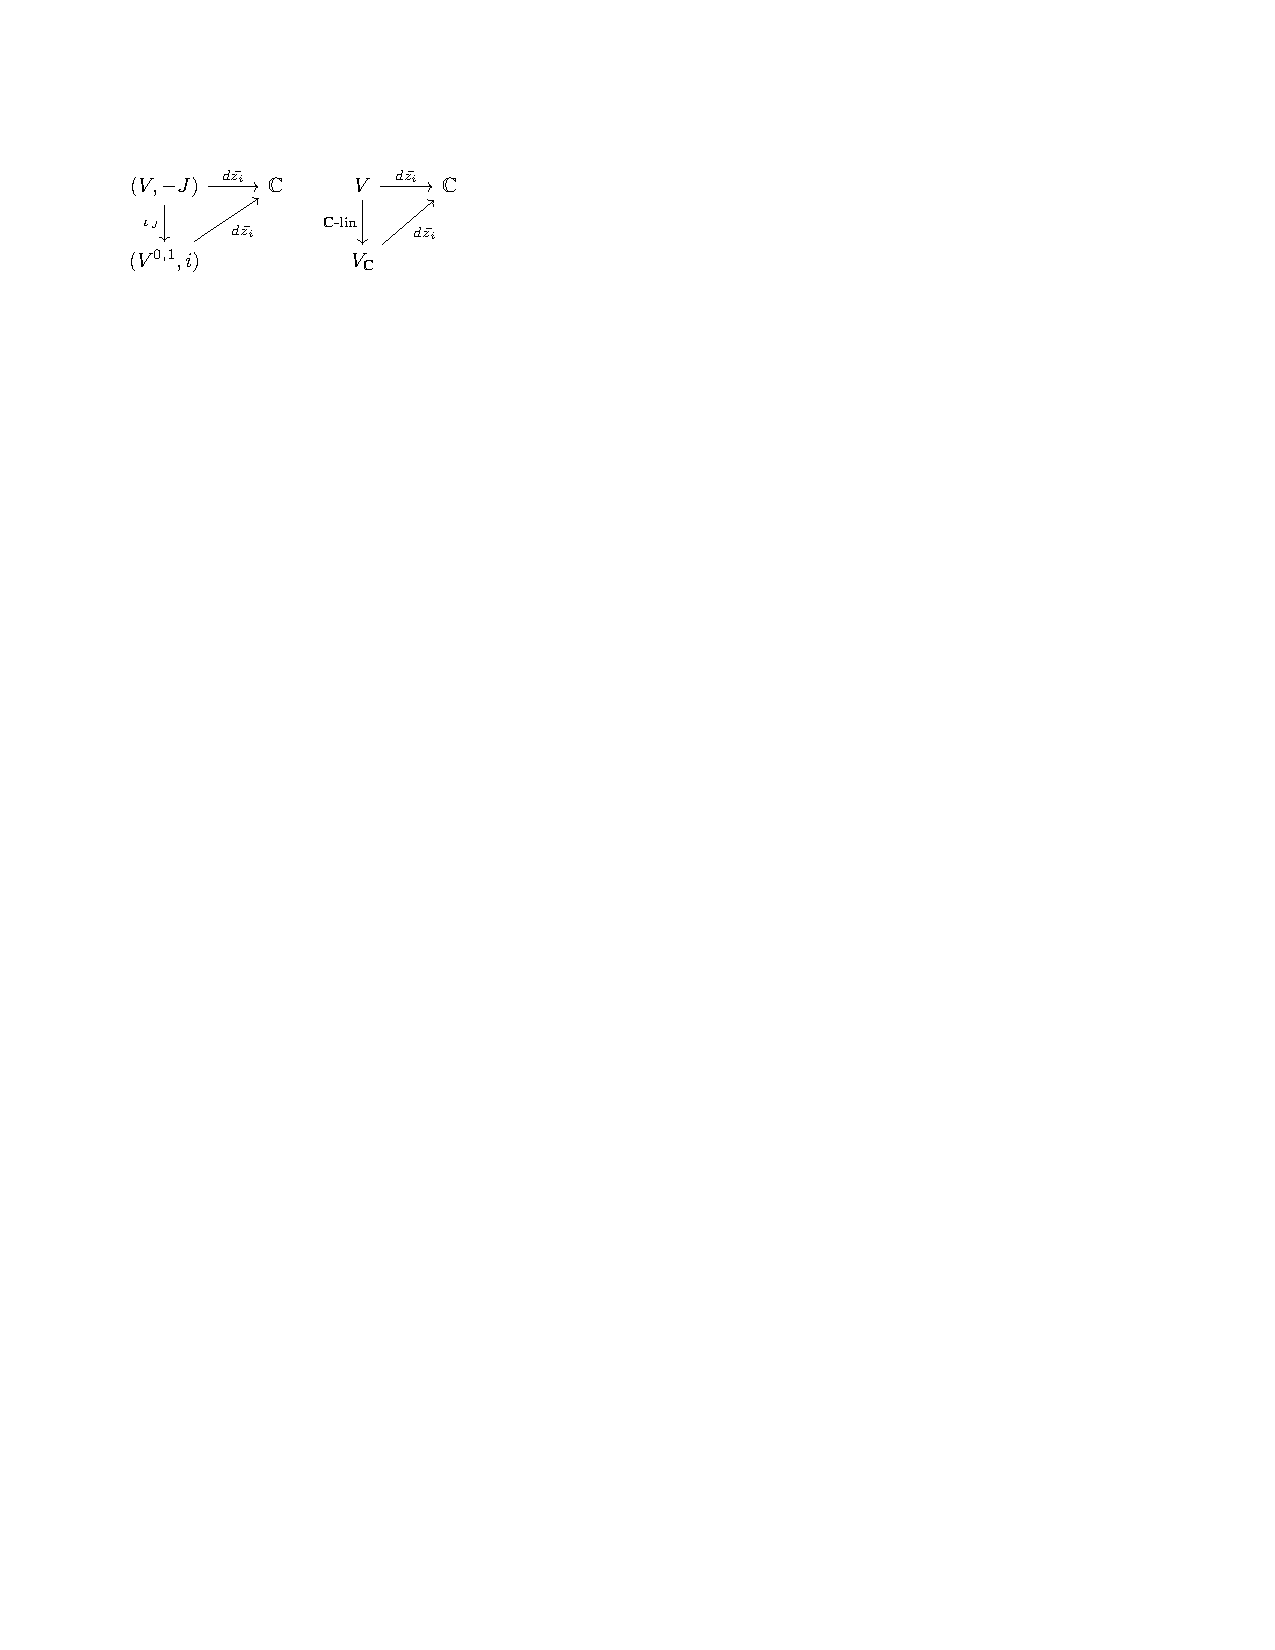
\includegraphics[width=.9\linewidth]{../img/fsa.pdf}
\caption{\label{fig:orgb175db8}
tikz caption}
\end{figure}
\end{document}